\documentclass{tufte-handout}
\usepackage{../braph2_dev}
\usepackage{graphicx, booktabs, array}
%\geometry{showframe} % display margins for debugging page layout

\title{Implement a new Property Panel}

\begin{document}

\maketitle

\begin{abstract}
\noindent
This is the developer tutorial for implementing a new property panel. 
In this tutorial, we will explain how to create the generator file \fn{*.gen.m} for a new property panel, which can then be compiled by \code{braph2genesis}. 
All property panels are (direct or indirect) extensions of the element \code{PanelProp}.
We will use the property panel \code{PanelPropLogical} as an example.
\end{abstract}

\tableofcontents

%%%%% %%%%% %%%%% %%%%% %%%%%
\clearpage
\section{Implementation of Property Panel (PanelPropLogical)}


To illustrate the general concepts of a property panel, we will start by implementing in detail the property panel \code{PanelPropLogical}, which is a direct extension of the element \code{PanelProp}.

\begin{lstlisting}[
	label=cd:m:panelproplogical:header,
	caption={
		{\bf PanelPropLogical element header.}
		The \code{header} section of the generator code for \fn{\_PanelPropLogical.gen.m} provides the general information about the \code{PanelPropLogical} element.
	}
]
%% ¡header!
PanelPropLogical < PanelProp (pr, panel property logical) plots the panel of a property logical.  ¥\circled{1}\circlednote{1}{The element \code{PanelPropLogical} is defined as a subclass of \code{PanelProp}. The moniker will be \code{pr}.}¥

%%% ¡description!
PanelPropLogical plots the panel for a LOGICAL property with a checkbox.
It works for all categories. ¥\circled{2}\circlednote{2}{Note that more specialized property panels do not necessarily need to work for all categories.}¥

\end{lstlisting}

\begin{lstlisting}[
	label=cd:m:panelproplogical:props_update,
	caption={
		{\bf PanelPropLogical element props update.}
		The \code{props\_update} section of the generator code for \fn{\_PanelPropLogical.gen.m} updates the properties of the \code{PanelProp} element. This defines the core properties of the property panel.
	}
]
%% ¡props_update!
...
%%% ¡prop!
EL (data, item) is the element.
%%%% ¡default!
PanelProp() ¥\circled{1}\twocirclednotes{1}{2}{define the default element and property for this property panel. This is necessary to ensure that the property panel refers to a property with the right format during unit testing.}¥

%%% ¡prop!
PROP (data, scalar) is the property number.
%%%% ¡default!
PanelProp.DRAW ¥\circled{2}¥
...
\end{lstlisting}

\begin{lstlisting}[
	label=cd:m:panelproplogical:props,
	caption={
		{\bf PanelPropLogical new props.}
		The \code{props} section of the generator code for \fn{\_PanelPropLogical.gen.m} defines the user interface (UI) objects and their callbacks for the \code{PanelPropLogical} element.
	}
]
%% ¡props!

%%% ¡prop!
CHECKBOX (evanescent, handle) is the logical value checkbox. ¥\circled{1}\circlednote{1}{defines the checkbox we need in the panel for a property logical. Note that this is of category EVANESCENT as it is initialized each time the code is run and is not saved.}¥
%%%% ¡calculate! ¥\circled{2}\circlednote{2}{initializes the UI object.}¥
el = pr.get('EL');
prop = pr.get('PROP');

checkbox = uicheckbox( ...
	'Parent', pr.memorize('H'), ... % H = p for Panel
	'Tag', 'CHECKBOX', ...
	'Text', '', ...
	'FontSize', BRAPH2.FONTSIZE, ...
	'Tooltip', [num2str(el.getPropProp(prop)) ' ' el.getPropDescription(prop)], ...
	'ValueChangedFcn', {@cb_checkbox} ...
	);

value = checkbox;
%%%% ¡calculate_callbacks! ¥\circled{3}\circlednote{3}{defines the callback for when the UI object is activated.}¥
function cb_checkbox(~, ~)
	el = pr.get('EL'); ¥\circle{4}\twocirclednotes{4}{5}{reteieve the element and property on which the callback operates.}¥
	prop = pr.get('PROP'); ¥\circle{4}¥

	checkbox = pr.get('CHECKBOX'); ¥\circled{5}\circlednote{5}{retrieves the UI object (in this case, a checkbox) and \circled{6} the new value.}¥
	new_value = logical(get(checkbox, 'Value')); ¥\circled{6}¥

	el.set(prop, new_value)  ¥\circled{7}\circlednote{7}{writes the new value of the logical property.}¥
end
\end{lstlisting}

\begin{lstlisting}[
	label=cd:m:panelproplogical:props_update2,
	caption={
		{\bf PanelPropLogical element props update (continued).}
		This continues the update of the \code{props\_update} section of the generator code for \fn{\_PanelPropLogical.gen.m}. Here, the essential properties to draw and manage the property panel are defined.
	}
]
%% ¡props_update!
...
%%% ¡prop!
X_DRAW (query, logical) draws the property panel. ¥\circled{1}\circlednote{1}{draws the panel. In this case, the property panel contains only a checkbox, memorized in \circled{2}.}¥
%%%% ¡calculate!
value = calculateValue@PanelProp(pr, PanelProp.X_DRAW, varargin{:}); % also warning
if value
	pr.memorize('CHECKBOX') ¥\circled{2}¥
end

%%% ¡prop!
DELETE (query, logical) resets the handles when the panel is deleted. ¥\circled{3}\circlednote{3}{resets the handles when the property panel and its UI objects when deleted. In this case, it erases the handle of the checkbox in \circled{4}.}¥
%%%% ¡calculate!
value = calculateValue@PanelProp(pr, PanelProp.DELETE, varargin{:}); % also warning
if value
	pr.set('CHECKBOX', Element.getNoValue()) ¥\circled{4}¥
end

%%% ¡prop!
HEIGHT (gui, size) is the pixel height of the property panel. ¥\circled{5}\circlednote{5}{specifies the height of the property panel.}¥
%%%% ¡default!
s(4)

%%% ¡prop!
REDRAW (query, logical) resizes the property panel and repositions its graphical objects. ¥\circled{6}\circlednote{6}{draws the property panel determining its graphical appearance. In this case, it just positions the checkbox in \circled{7}.}¥
%%%% ¡calculate!
value = calculateValue@PanelProp(pr, PanelProp.REDRAW, varargin{:}); % also warning
if value
	w_p = get_from_varargin(w(pr.get('H'), 'pixels'), 'Width', varargin);

	set(pr.get('CHECKBOX'), 'Position', [s(.3) s(.3) .70*w_p s(1.75)]) ¥\circled{7}¥
end

%%% ¡prop!
UPDATE (query, logical) updates the content and permissions of the checkbox. ¥\circled{8}\circlednote{8}{updates the status of the UI objects within the panel based on the current state of the element and property to which it is linked. In this case, it just sets the value and permissions of the checkbox.}¥
%%%% ¡calculate!
value = calculateValue@PanelProp(pr, PanelProp.UPDATE, varargin{:}); % also warning
if value

	el = pr.get('EL'); ¥\circled{9}\twocirclednotes{9}{10}{retrieve the element and property to which the property panel refer.}¥
	prop = pr.get('PROP'); ¥\circled{10}¥

	switch el.getPropCategory(prop) ¥\circled{11}\circlednote{11}{switches between the different possible property categories to make this property panel work for all of them. More specialized property panels might not need to work for all category, thus simplifying this code.}¥
		case Category.CONSTANT ¥\circled{12}\circlednote{12}{When the property is a \code{CONSTANT}, the checkbox is disabled as it cannot be changed.}¥
			set(pr.get('CHECKBOX'), ...
				'Value', el.get(prop), ...
				'Enable', 'off' ...
			)

		case Category.METADATA ¥\circled{13}\circlednote{13}{When the property is a \code{METADATA}, the \code{CHECKBOX}'s enabled status depends on whether it is locked.}¥
			set(pr.get('CHECKBOX'), 'Value', el.get(prop))

			if el.isLocked(prop)
				set(pr.get('CHECKBOX'), 'Enable', 'off')
			end

		case {Category.PARAMETER, Category.DATA, Category.FIGURE, Category.GUI}  ¥\circled{14}\circlednote{14}{When the property is \code{PARAMETER}, \code{DATA}, \code{FIGURE}, or \code{GUI}, the checkbox is enabled only when the property is not locked or a callback.}¥
			set(pr.get('CHECKBOX'), 'Value', el.get(prop))

			prop_value = el.getr(prop);
			if el.isLocked(prop) || isa(prop_value, 'Callback')
				set(pr.get('CHECKBOX'), 'Enable', 'off')
			end

		case {Category.RESULT Category.QUERY Category.EVANESCENT} ¥\circled{15}\circlednote{15}{When the property is \code{RESULT}, \code{QUEY}, or \code{EVANESCENT}, the checkbox is not enabled and it visualizes the default value if the property has not been calculated yet.}¥
			prop_value = el.getr(prop);

			if isa(prop_value, 'NoValue')
				set(pr.get('CHECKBOX'), 'Value', el.getPropDefault(prop))
			else
				set(pr.get('CHECKBOX'), 'Value', el.get(prop))
			end

			set(pr.get('CHECKBOX'), 'Enable', 'off')
	end
end
\end{lstlisting}

%%%%% %%%%% %%%%% %%%%% %%%%%
\clearpage

\section{Example Property Panels for Various UI Objects}

The implementation of \code{PanelPropLogical} shown in the previous section can be extended to all other user interface (UI) objects. There are several examples already available in the core code of BRAPH~2.0, each coupled with its corresponding property panel as an example, as shown in the table below. These can be used to guide the realization of new property panels.

\newcommand{\addpicbutton}{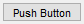
\includegraphics[width=6em]{fig01.png}}
\newcommand{\addpiccheckbox}{
\includegraphics[width=6em]{fig02.png}}
\newcommand{\addpiceditfield}{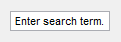
\includegraphics[width=6em]{fig03.png}}
\newcommand{\addpicslider}{
\includegraphics[width=6em]{fig04.png}}
\newcommand{\addpiclistbox}{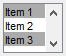
\includegraphics[width=6em]{fig05.png}}
\newcommand{\addpicdropdown}{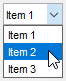
\includegraphics[width=6em]{fig06.png}}
\newcommand{\addpictextarea}{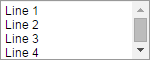
\includegraphics[width=6em]{fig07.png}}
\newcommand{\addpiccontextmenu}{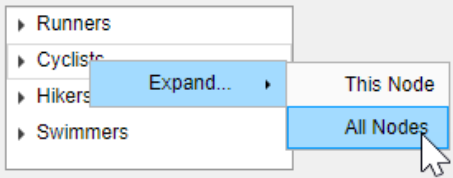
\includegraphics[width=6em]{fig08.png}}
\newcommand{\addpictable}{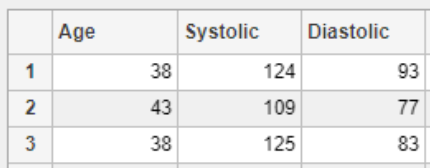
\includegraphics[width=6em]{fig09.png}}
\newcommand{\addpicgauge}{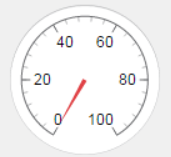
\includegraphics[width=6em]{fig10.png}}
\newcommand{\addpicradiobutton}{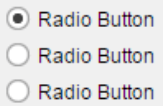
\includegraphics[width=6em]{fig11.png}}
\newcommand{\addpicspinner}{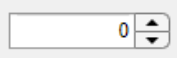
\includegraphics[width=6em]{fig12.png}}
\newcommand{\addpictogglebutton}{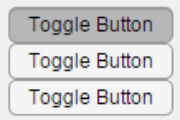
\includegraphics[width=6em]{fig13.png}}
\newcolumntype{C}{>{\centering\arraybackslash}m{12em}}
\begin{table}\sffamily
	\begin{tabular}{l*4{C}@{}}
		\toprule
		UI Object & Example & Exemple PanelProp \\ 
		\midrule
		uibutton & \addpicbutton & PanelPropItem \\ 
		uicheckbox & \addpiccheckbox & PanelPropLogical \\ 
		uitextarea  & \addpictextarea & PanelPropStringList \\
		uieditfield & \addpiceditfield & PanelPropString \\
		uidropdown & \addpicdropdown & PanelPropOption \\
		uicontextmenu & \addpiccontextmenu & PanelPropMatrix \\
		uitable & \addpictable & PanelPropMatrix \\
		uilistbox & \addpiclistbox & PanelPropClassList \\
		uislider & \addpicslider & PanelPropCell \\
		uigauge & \addpicgauge & Not yet implemented \\
		uiradiobutton & \addpicradiobutton & Not yet implemented \\
		uispinner & \addpicspinner & Not yet implemented \\
		uitogglebutton & \addpictogglebutton & Not yet implemented \\
		\bottomrule \\
	\end{tabular}
\end{table} 

%\bibliography{biblio}
%\bibliographystyle{plainnat}

\end{document}